\chapter{Deterministic discrete time models}

In Section~\ref{sec:DE_logistic}, the discrete time logistic equation was studied, and some theory for difference equations was presented in Chapter~\ref{chap:theory_discrete_time}. Here, we give several examples, more or less detailed, of the use of discrete time systems.

The population dynamics of single species with seasonal
reproduction and first-order feedback are often modelled
using a single difference equation, so our first few models are of this type.


\section{Other applications of the logistic map}
Here, we list a few contexts in which the logistic map has been used, besides the growth of the human population.
\subsection{Tumor cell growth}
A population of tumor cells $N(t)$ growing in a container can be modeled using a logistic map. Here, $r$ is the rate of growth of the tumor cells. Normalization of $N(t)$ means that $N(t)$ represents the fraction of the total population of cells contained in the cell culture. The cell culture can support a maximal number of cells represented by 1. The main assumption of the model is that the growth rate is constant.


\section{Bacteria population}
E. coli are able to divide every 20 minutes under optimal conditions. Describe the temporal evolution of a colony of E. coli.


\begin{definition}
Cell division is the process by which a cell, called the parent cell, divides into two cells, called daughter cells. Cell division is usually a small segment of a larger cell cycle.
\begin{itemize}
\item Prokaryotic cells: binary fission
\item Eukaryotic cells: mitosis+cytokinesis
\end{itemize}
\end{definition}

\begin{definition}
Binary fission: The prokaryotic chromosome is a single DNA molecule that first replicates, then attaches each copy to a different part of the cell membrane. When the cell begins to pull apart, the replicate and original chromosomes are separated. Following cell splitting (cytokinesis), there are then two cells of identical genetic composition (except for the rare chance of a spontaneous mutation).
\end{definition}
\begin{center}
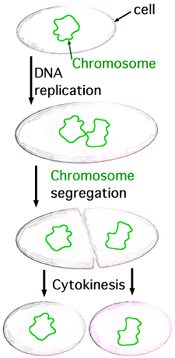
\includegraphics[width=.25\textwidth]{figs_steph/Binary_fission}
\end{center}



\begin{definition}
Mitosis+Cytokinesis: Mitosis is the process by which a cell separates its duplicated genome into two identical halves. It is generally followed immediately by cytokinesis which divides the cytoplasm and cell membrane. This results in two identical daughter cells with a roughly equal distribution of organelles and other cellular components. Mitosis and cytokinesis together is defined as the mitotic (M) phase of the cell cycle, the division of the mother cell into two daughter cells, each the genetic equivalent of the parent cell.
\end{definition}
\begin{center}
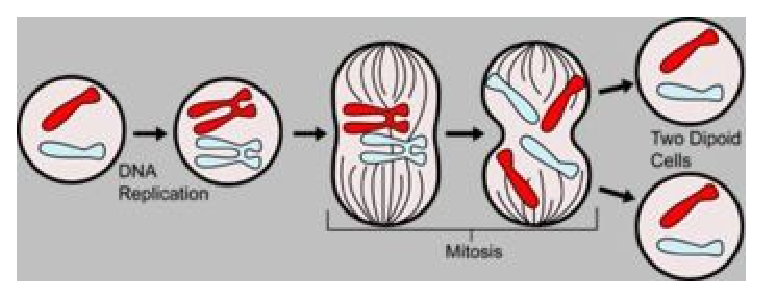
\includegraphics[width=.8\textwidth]{figs_steph/Mitosis}
\end{center}

Organisms that reproduce by binary fission (asexual reproduction) exhibit exponential growth. If organisms (or cells) are synchronized, the formalism of difference equation can be used.
The model (for an unlimited environment) to describe the temporal evolution of the E. Coli colony is expressed as
$$x_{t+1}=2x_t, \quad t=0,1,2,\dots$$
where $x_t$ is the state variable that represents the number of cells at the generation $t$. If the initial population $x_0$ is known then the solution is unique and is 
$$x_{t}=2^tx_0, \quad t=0,1,2,\dots$$

The asymptotic behavior of the solution is
$$\lim_{t\rightarrow \infty} x_t=\infty$$
as $a=2>1$. 
Note: If differential equation formalism was used
$$\frac{dx}{dt}=\frac{1440}{20}x$$
the solution would be $x(t)=x_0e^{\frac{1440}{20}t}$.



\section{The Ricker model}
another model for describing a population $N(t)$ in a limited environment
$$N(t+1)=N(t)\exp\left\{r\left(1-\frac{N(t)}{K}\right) \right\}=f(N(t)),$$
where $r$ is the intrinsic growth rate and $K$ is the carrying capacity. The growth rate $f(N(t))$ is increasing  in $N(t)$ and the per capita growth $\frac{f(N)}{N}$ is decreasing in $N(t)$. The increase in population is not sufficient to compensate for the decrease in the per capita growth, then $\lim_{N(t)\rightarrow +\infty}f(N(t))=0$. Then the Ricker model can be referred as to overcompensatory.
\begin{itemize}
\item $r < 2$ Globally asymptotically stable equilibrium $\bar x=K$
\item r = 2 Bifurcation into a stable 2-cycle
\item r = 2.5 Bifurcation into a stable 4-cycle
\item Then there is a series of cycle duplication: 8-cycle, 16-cycle, etc.
\item r = 2.692 Chaos 
\item For $r > 2.7$ there are some regions where dynamics returns to a cycle, e.g., r=3.15. 
\end{itemize}



\section{The Hassell model}
A population $N(t)$ in a limited environment
$$N(t+1)=\frac{rN(t)}{(1 + N(t))^b}$$
where $r$ is the intrinsic growth rate for small populations and b represents the inhibitive density-dependent feedback, usually attributed to the environment. 



\section{The Beverton-Holt model}
$$N(t+1)=\frac{ e ^r K N(t)}{K + (e^r -1)N(t)}$$
with $r$ is the intrinsic growth rate, the carrying capacity is $K$.

\section{Example of a 2-dimensional system}
\begin{equation*}
\begin{array}{cl}
x(t+1)=&x(t)(a-x(t)-y(t)), \quad a>0\\
y(t+1)=&y(t)(b+x(t)), \quad 0<b<1.
\end{array}
\end{equation*}


To find equilibria, solve the fixed point problem for $x$ and $y$,
\begin{equation*}
\begin{array}{cl}
x=&x(a-x-y)\\
y=&y(b+x)
\end{array}
\end{equation*}
We find 3 equilibria:
\[
(\bar x_1, \bar y_1)=(0,0), \quad  (\bar x_2, \bar y_2)=(a-1,0), \quad (\bar x_3, \bar y_3)=(1-b,a+b-2).
\]
The Jacobian of the system is
\[
J=\begin{pmatrix}
a-2x-y & -x \\
y & b+x
\end{pmatrix}.
\]
The Jacobians evaluated at each equilibrium are:
$$
J_{(\bar x_1, \bar y_1)}=\left ( 
\begin{array}{cc}
a & 0 \\
0 & b
\end{array}
\right ) \quad 
J_{(\bar x_2, \bar y_2)}=\left ( 
\begin{array}{cc}
2-a & 1-a \\
0 & b+a-1
\end{array}
\right ) \quad
J_{(\bar x_3, \bar y_3)}=\left ( 
\begin{array}{cc}
b & -1+b \\
a+b-2 & 1
\end{array}
\right )
$$
\begin{itemize}
\item Eigenvalues of $J_{(\bar x_1, \bar y_1)}$ are $a$ and $b$. By definition $|b|<1$. If $a<1$, $(\bar x_1, \bar y_1)$ is L.A.S.
\item $(\bar x_2, \bar y_2)=(a-1,0)$ exists only if $1<a$. Eigenvalues of $J_{(\bar x_2, \bar y_2)}$ are $2-a$ and $b+a-1$, then the stability of $(\bar x_2, \bar y_2)$ depends on $|2-a|<1$ and $|b+a-1|<1$. These inequalities lead to $1<a<2-b$.
\item From Theorem \ref{theo:stable2dim}, $(\bar x_3, \bar y_3)$ is L.A.S. if 
$$|1+b|<1+b-(-1+b)(a+b-2)<2.$$
$(\bar x_3, \bar y_3)$ is positive if $b<1$ and $a+b>2$. Then the biological existence and the LAS of $(\bar x_3, \bar y_3)$ are possible for
$$2<a+b<3.$$
\end{itemize}


\section{An SIR epidemic model}
Epidemic models were introduced in Section~\ref{sec:epid_residence_time}, and will be further discussed in Chapter~\ref{chap:epidemic_models} (in the ODE case). We refer in particular to Chapter~\ref{chap:epidemic_models}, where much more details can be found.

Here, we present an example of SIR model in difference equation formalism.
\begin{figure}[h]
%\includegraphics[width=0.8\textwidth]{figs_steph/SIR}
\caption{SIR model: disease with recovery and permanent immunity, here birth=death=b.}
\end{figure}
\begin{align}
S(t+1) &= S(t)-\beta \dfrac{S(t)}{N}I(t) +b(I(t)+R(t))\\
I(t+1) &= (1-\gamma -b)I(t)+\beta \dfrac{S(t)}{N}I(t)\\
R(t+1) &= R(t)(1-b)+\gamma I(t),
\end{align}
where $N=S(0)+I(0)+R(0)$. Parameters are $\beta$, the contact number (the average number of successful contacts made by one infected individual during the time $t$ to $t+1$), $b=d$, the rate of birth and death, $\gamma$, the rate of recovery ($1/\gamma $ is the average length of the infectious period when there are no death, $1/(\gamma +b)$ is the average length of the infectious period when deaths are included).

It is easy to check that the total population is constant, $N=S(t)+I(t)+R(t)$.
Also, solutions are nonnegative if $b,\gamma>0$ and
$$0<b+\gamma <1, \qquad 0<\beta <1$$.

We now consider the reduced system where $R(t)=N-I(t)-S(t)$ (which can be done since the total population is constant):
\begin{align*}
S(t+1)&=S(t)-\beta \dfrac{S(t)}{N}I(t) +b(N-S(t))\\
I(t+1)&=(1-\gamma -b)I(t)+\beta \dfrac{S(t)}{N}I(t).
\end{align*}
We find two equilibria: the disease-free equilibrium $(S_1,I_1)=(N,0)$ and the endemic equilibrium $(S_2,I_2)=\left (N\frac{(\gamma+b)}{\beta},bN\frac{\beta - (\gamma + b)}{\beta (\gamma +b)}\right)$.

\subsection{Stability of the disease free equilibrium $(S_1,I_1)$}
The Jacobian evaluated at $(S_1,I_1)$ is
$$
J(S_1,I_1)=\left (
\begin{array}{cc}
1-b & -\beta \\
0 & 1-b-\gamma +\beta 
\end{array}
\right )
$$
as the Jacobian is upper triangular its eigenvalues are
$$\lambda _1 = 1-b , \quad \lambda _2= 1-b-\gamma +\beta  .$$
$(S_1,I_1)$ is locally asymptotically stable if $|\lambda_{1,2}|<1$
\begin{itemize}
\item from assumptions, we have $0<\lambda _1 <1$
\item if $\frac{\beta}{\gamma +b}<1$ (where $\mathcal{R}_0=\frac{\beta}{\gamma +b}$ is the basis reproduction number), $0<\lambda _2 <1$
\end{itemize}
if $\mathcal{R}_0 <1$, there exist only one (biologically plausible) equilibrium, the disease-free equilibrium, and it is L.A.S. (see Figure \ref{fig:SIRsimul})


\subsection{Stability of the endemic equilibrium $(S_2,I_2)$}
The Jacobian evaluated at $(S_2,I_2)$ is
$$
J(S_2,I_2)=\left (
\begin{array}{cc}
1-b\mathcal{R}_0 & -\beta/\mathcal{R}_0 \\
b(\mathcal{R}_0-1) & 1
\end{array}
\right )
$$
where $\tr(J(S_2,I_2))=2-b\mathcal{R}_0 $ (assume $ \tr(J(S_2,I_2))\geq 0$), and $\det(J(S_2,I_2))=1-b\mathcal{R}_0+\beta b (1-\frac{1}{\mathcal{R}_0})$.


Condition for L.A.S (Theorem \ref{theo:stable2dim})
$$2-b\mathcal{R}_0 <2-b\mathcal{R}_0+\beta b (1-\frac{1}{\mathcal{R}_0}) <2$$
this condition is satified because
$$\beta (1-1/\mathcal{R}_0)<1<\mathcal{R}_0$$

If $1<\mathcal{R_0}\leq 2/b$, the endemic equilibrium  exists and it is L.A.S. (see Figure \ref{fig:SIRsimul}).

%\begin{figure}[h]
%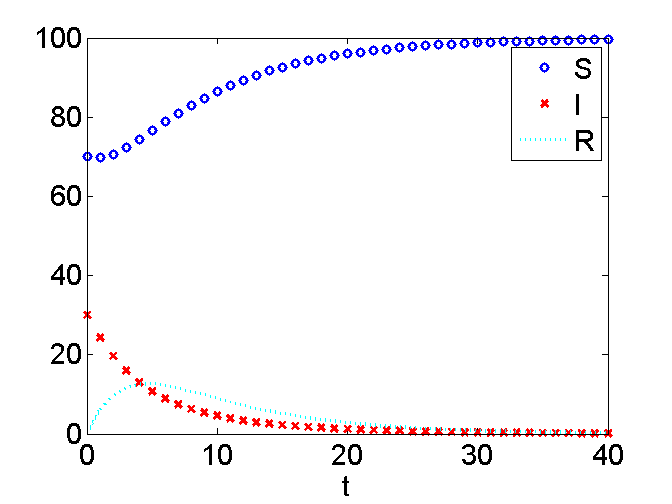
\includegraphics[width=.49\textwidth]{figs_steph/R1}
%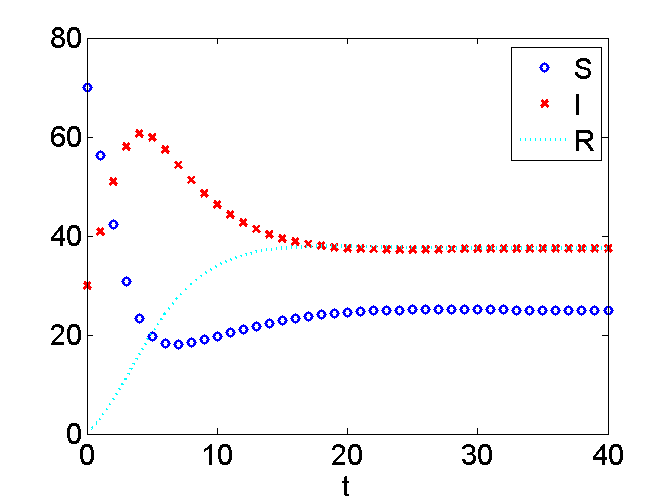
\includegraphics[width=.49\textwidth]{figs_steph/R4}
%\label{fig:SIRsimul}
%\caption{SIR model: {\bf Left)} $R_0=0.75$ the disease-free equilibrium is L.A.S. {\bf Right)} $R_0=4$ the endemic equilibrium is L.A.S}
%\end{figure}


\section{Predator-Prey models}
{\bf Assumptions}
\begin{itemize}
\item the prey has unlimited resources
\item the prey's only threat is the predator
\item the predator is a specialist; i.e., the predator's only food supply is the prey
\item predator growth depends on the prey it catches
\end{itemize}
{\bf Variables}
\begin{itemize}
\item $N(t)$ number of preys
\item $P(t)$ number of predators
\end{itemize}
{\bf Parameters}
\begin{itemize}
\item $r$ intrinsic rate of growth of prey
\item $d$ rate of death of predators
\item $eP(t)$ per capita prey reduction due to predation
\item $bN(t)$ per capita predator increase due to prey
\end{itemize}
\begin{equation*}
\begin{array}{cl}
N(t+1)=&(1+r)N(t)-e N(t)P(t)\\
P(t+1)=&(1-d)P(t)+bN(t)P(t)
\end{array}
\end{equation*}

{\bf Neubert and Kot model:}
If the prey follows a logistic growth
\begin{equation*}
\begin{array}{cl}
N(t+1)=&N(t)+rN(t)\left ( 1-\frac{N(t)}{K} \right ) -e N(t)P(t)\\
P(t+1)=&(1-d)P(t)+bN(t)P(t)
\end{array}
\end{equation*}




\section{Structured population models}
Structured population models are used when the population can be organized or divided into various subclasses following traits such as age, life-stage or size. The variable that describes this trait is called the structuring variable.
\begin{itemize}
\item In age-structured model, the  population is subdivided into age groups. For the human population, for example, age groups may be 5 year lengths, 0-5, 5-10, $\dots$, or 1 year lengths.
\item In stage-structured model, the population is organized into developmental stage: juveniles and adults, or for insects, egg, larva, pupa and adult.
\item In size-structured  model, individuals in the population are grouped according to size (length, weight, biomass).
\end{itemize}
The dynamic interactions among the stages, ages or sizes determine how the population structure changes over the time. Other structuring variables can be taken into account: sex and space.




\section{Leslie matrix model}
The Leslie Matrix (also called the Leslie Model) describes the growth of populations with structure (and their projected age distribution); the population is closed to migration and only one sex, usually the female, is considered.


Assume the population is closed to migration and only the females are modeled. Males are presented, but are not specifically modeled (when the sex ratio of males to females is $a/b$ and the survival rate per age group is the same for males and females, then the number of males equals the number of females times $a/b$). 


Let the total number of age groups is $m$ ($m$ the last reproductive age). During the interval of time $t$ and $t+1$ individuals age from $i$ to $i+1$: time interval coincides with the age interval.
\begin{itemize}
\item $x_i(t)$ number of females in the $i^{th}$ age group at time $t$.
\item $b_i$ average number of newborn females produced by one females in the $i^{th}$ age group that survive through the time interval in which they were born, $b_i\geq 0$
\item $s_i$ fraction of the $i^{th}$ age group that lives  to the $(i+1)st$ age, $0<s_i\leq 1$
\end{itemize}
\begin{figure}
\begin{center}
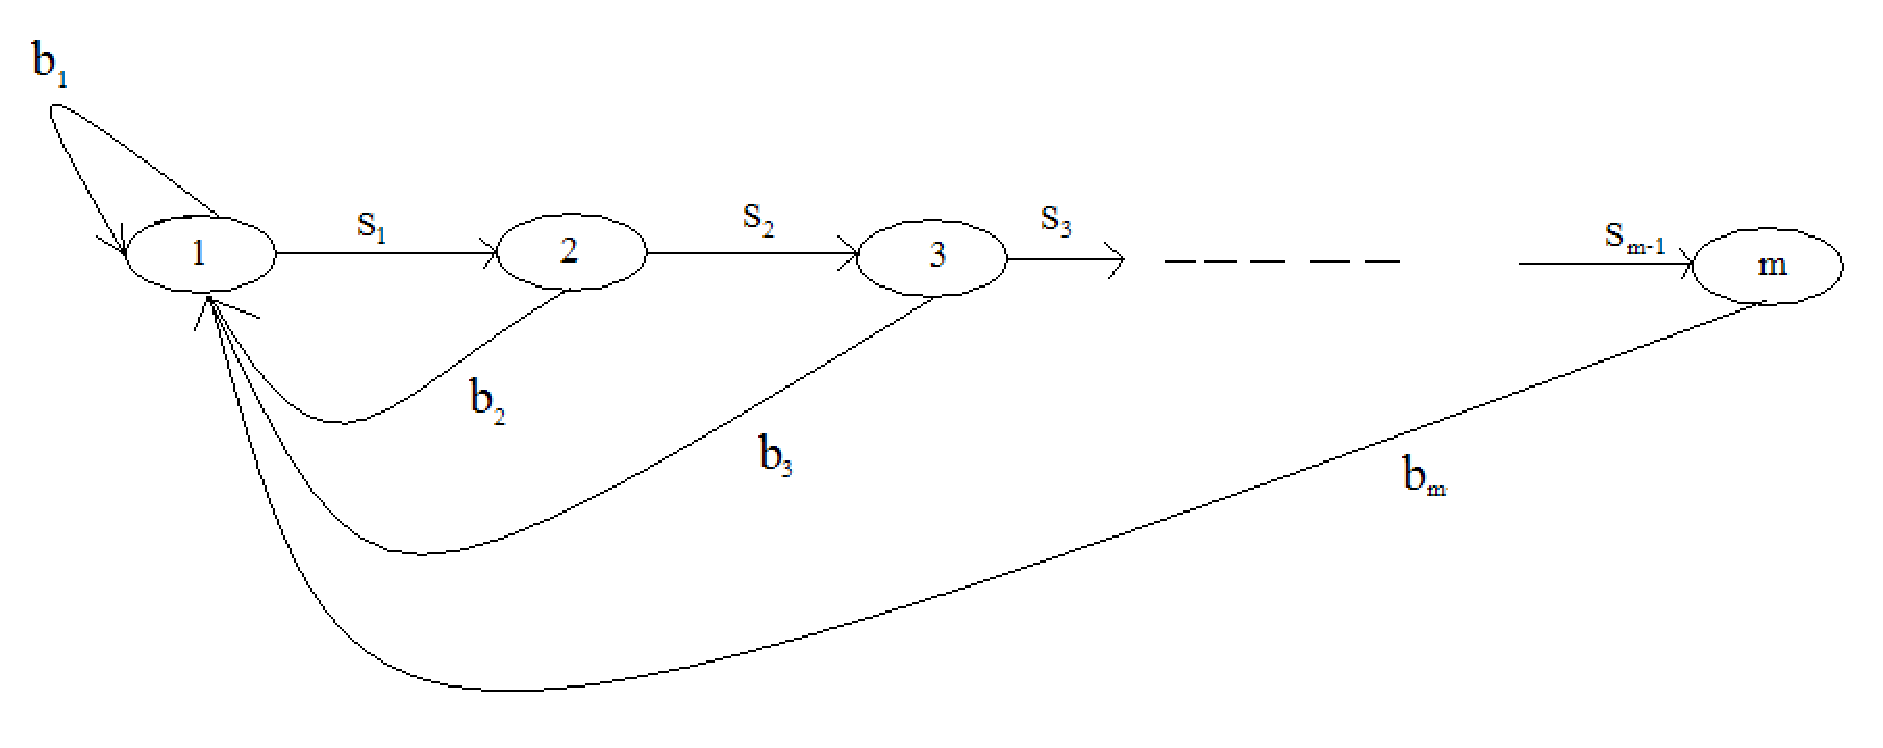
\includegraphics[width=0.6\textwidth]{figs_steph/LesliePattern}
\caption{Life cycle graph of the Leslie matrix on $m$ age classes: each node represents each age group $x_i$, and arcs represent relation between two groups. An arrow connects the node $j$ to $i$ if the $ij^{th}$ element in the Leslie matrix $L$ is nonzero.}
\end{center}
\end{figure}

\begin{subequations} 
\begin{align}
x_{1}(t+1)=& b_1 x_1(t)+b_2x_2(t)+b_3x_3(t)+\dots b_mx_m(t)\label{eq:Leslie1}\\
x_{2}(t+1)=&s_1 x_1(t)& \label{eq:Leslie2}\\
x_{3}(t+1)=&s_2 x_2(t)& \label{eq:Leslie3}\\
\vdots &\\
x_{m}(t+1)=&s_{m-1} x_{m-1}(t)& \label{eq:Leslie3}\\
\end{align}   
\end{subequations} 
Using matrix notation,
\begin{equation}
X(t+1)=\left (
\begin{array}{c}
x_1(t+1)\\
x_2(t+1)\\
x_3(t+1)\\
\vdots\\
x_m(t+1)
\end{array}
\right )
=
\left(
\begin{array}{ccccc}
b_1 & b_2 & \hdots & b_{m-1} & b_m\\
s_1 & 0  & \hdots & 0 & 0\\
0 & s_2  & \hdots & 0 & 0\\
\vdots & \vdots & \ddots & \vdots & \vdots \\
0 &0 &\hdots & s_{m-1} &0
\end{array}
\right)
\left (
\begin{array}{c}
x_1(t)\\
x_2(t)\\
x_3(t)\\
\vdots\\
x_m(t)
\end{array}
\right )=LX(t)
\end{equation}
where $L$ is called the Leslie matrix: fertilities or fecundities on the first row and survival probabilities on the subdiagonal. All other entries in the Leslie matrix are zero.



$$X(1)=LX(0)$$
$$X(2)=LX(1)=L\left(LX(0)\right)=L^2X(0)$$
In general
$$X(t)=L^tX(0)$$







\begin{definition}
A Leslie matrix is a nonnegative matrix.
\end{definition}




A necessary condition for a Leslie matrix to be irreductible is $b_m\not =0$.


Frobenius Theorem gives sufficient conditions that guarantees the Leslie matrix has one positive strictly dominant eigenvalue.


If the Leslie matrix satisfies $L^p>0$ for some positive integer $p$, then $L$ is primitive. Then, the Frobenius Theorem states that in this case L has a unique strictly dominant eigenvalue $\lambda _1$ satisfying $|\lambda _1|>|\lambda _i|$, for $j\not =1$, that is positive. Associated with the strictly dominant eigenvalue $\lambda _1$ is a positive eigenvector $V_1$, that is referred to as a stable age distribution.


Assume matrix $L$ is irreductible and primitive and $m$ eigenvectors form a linearly independent set; then the solution to
$$X(t+1)=LX(t)$$
can be written
$$X(t)=L^tX(0)=\sum_{i=1}^m c_i \lambda _i ^t V_i$$
where $\lambda _1$ is the strictly dominant eigenvalue. Dividing the solution by $\lambda _1^t$ gives
$$\frac{X(t)}{\lambda _1^t}=\frac{L^tX(0)}{\lambda _1^t}=c_1 V_1 + \frac{c_2 \lambda _2 ^t}{\lambda _1^t} V_2+\dots + \frac{c_m \lambda _m ^t}{\lambda _1^t} V_m $$
As $|\lambda _i/\lambda_1|<1$, $(\lambda _i/\lambda_1)^t\rightarrow 0$ as $t\rightarrow +\infty$. Thus
$$\lim_{t\rightarrow +\infty} \frac{X(t)}{\lambda _1^t}=\lim_{t\rightarrow +\infty}  \frac{L^tX(0)}{\lambda _1^t}=c_1V_1 .$$
Hence after many generations, $X(t)=L^tX(0)=c_1\lambda _1^tV_1$. The population size either increasing ($\lambda _1 >1$) or decreasing ($\lambda _1 <1$) geometrically as $t$ goes larger.

The population distribution $X(t)/\lambda _1 ^t$ approaches a constant multiple of the eigenvector $V_1$; thus $V_1$ is referred to as a stable age distribution. It means that for large values of time, the age distribution vector is a scalar multiple of the eigenvector associated with the largest eigenvalue of the matrix. Consequently the proportion of females in each of the age classes becomes constant, these limiting proportions can be determined from the eigenvector $V_1$.

An explicit expression for $V_1$ in the case of a Leslie matrix is \cite{Pielou1977}
\begin{equation}
\label{eq:Eigenvector}
V_1=\left (\begin{array}{c}
1\\
\frac{s_1}{\lambda _1}\\
\vdots\\
\frac{s_1s_2\dots s_{m-2}}{\lambda_1^{m-2}}\\
\frac{s_1s_2\dots s_{m-1}}{\lambda_1^{m-1}}
\end{array}\right )
\end{equation}


The characteristic equation for the Leslie matrix satisfies $\det(L-\lambda I)=0$ or
$$\det 
\left(
\begin{array}{ccccc}
b_1-\lambda & b_2 & \hdots & b_{m-1} & b_m\\
s_1 & -\lambda  & \hdots & 0 & 0\\
0 & s_2  & \hdots & 0 & 0\\
\vdots & \vdots & \ddots & \vdots & \vdots \\
0 &0 &\hdots & s_{m-1} &-\lambda
\end{array}
\right)=0$$
or
$$p(\lambda)=\lambda ^m-b_1 \lambda^{m-1}-b_2s_1 \lambda^{m-2}- b_3s_1 s_2 \lambda^{m-3}-\dots - b_m s_1s_2 s_3\dots s_{m-1}=0 $$
From Descarte's Rule, since there is only one change in sign in the polynomial, $p(\lambda)$ has one positive real root, that is the dominant eigenvalue $\lambda _1$.

How is the dominant eigenvalue $\lambda _1$: $\lambda _1 >1$ or $\lambda _1 <1$?
\begin{itemize}
\item $\lim _{\lambda \rightarrow \infty}p(\lambda)=\infty$
\item $p(0)<0$
\item $p(\lambda)$ crosses the positive $\lambda-$axis only once at $\lambda_1$
\end{itemize}
then 
\begin{itemize}
\item $\lambda _1 >1$ $\Leftrightarrow$ $p(1)<0$
\item $\lambda _1 <1$ $\Leftrightarrow$ $p(1)>0$
\end{itemize}
where $p(1)=1-b_1 -b_2s_1 - b_3s_1 s_2 -\dots - b_m s_1s_2 s_3\dots s_{m-1}$, and $p(1)=1-R_0$.
Hence
\begin{itemize}
\item $\lambda _1 >1$ $\Leftrightarrow$ $1<R_0$
\item $\lambda _1 <1$ $\Leftrightarrow$ $1>R_0$
\end{itemize}

\begin{definition}
The reproductive number $R_0$ is the average number of offspring produced by an
individual in its lifetime:
$$R_0=b_1+b_2s_1+b_3s_1s_2+\dots+b_ms_1s_2\dots s_{m-1}$$
where each term represent the average
number of offsprings produced by individuals of age $i$.
\begin{itemize}
\item $R_0 < 1$ individuals not fully replacing themselves, population shrinking
\item $R_0 = 1$ individual exactly replacing themselves, population size stable
\item $R_0 > 1$ individuals more than replacing themselves, population growing
\end{itemize}
\end{definition}


\begin{theorem}
Assume the Leslie matrix $L$ defined as
$$X(t+1)=\left (
\begin{array}{c}
x_1(t+1)\\
x_2(t+1)\\
x_3(t+1)\\
\vdots\\
x_m(t+1)
\end{array}
\right )
=
\left(
\begin{array}{ccccc}
b_1 & b_2 & \hdots & b_{m-1} & b_m\\
s_1 & 0  & \hdots & 0 & 0\\
0 & s_2  & \hdots & 0 & 0\\
\vdots & \vdots & \ddots & \vdots & \vdots \\
0 &0 &\hdots & s_{m-1} &0
\end{array}
\right)
\left (
\begin{array}{c}
x_1(t)\\
x_2(t)\\
x_3(t)\\
\vdots\\
x_m(t)
\end{array}
\right )=LX(t)
$$
is irreductible and primitive. The characteristic polynomial of $L$ i given by
$$p(\lambda)=\lambda ^m-b_1 \lambda^{m-1}-b_2s_1 \lambda^{m-2}- b_3s_1 s_2 \lambda^{m-3}-\dots - b_m s_1s_2 s_3\dots s_{m-1}=0 .$$
Matrix $L$ has a strictly dominant eigenvalue $\lambda _1>0$ satisfying the following relationships:
\begin{itemize}
\item $\lambda _1 =1$ if and only if $R_0=1$,
\item $\lambda _1 <1$ if and only if $R_0<1$,
\item $\lambda _1 >1$ if and only if $R_0>1$,
\end{itemize}
where $R_0$ is the inherent reproductive number defined by
$$R_0=b_1+b_2s_1+b_3s_1s_2+\dots+b_ms_1s_2\dots s_{m-1}.$$
In addition the stable age distribution $V_1$ satisfies
$$V_1=\left (\begin{array}{c}
1\\
\frac{s_1}{\lambda _1}\\
\vdots\\
\frac{s_1s_2\dots s_{m-2}}{\lambda_1^{m-2}}\\
\frac{s_1s_2\dots s_{m-1}}{\lambda_1^{m-1}}
\end{array}\right ).
$$
\end{theorem}

\subsection{Salmon population}
Suppose a population of salmon live to three years of age. Each adult salmon produces 800 offspring. The
probability of a salmon surviving the first year to live on to the second year is $5\%$, and the probability of a
salmon surviving the second year to live on to the third year is $2.5\%$.
\begin{itemize}
\item Find the Leslie matrix for this population.
\item If there are 10 females in each of the three age classes, find the initial age distribution vector. Use Matlab
to find the population age distribution vectors for each of the first 100 years.
\item Use Matlab to find the eigenvalues and eigenvectors of the Leslie Matrix. Is there a strictly dominant eigenvalue?
\item Describe what happens to this population of salmon over time?
\end{itemize}

\subsection{Human Population}
Suppose the population of the United States is broken up into ten 5-year age classes. The values for the
reproduction rates $F_i$ and the survival rates $P_i$ for each age class are shown in the table below.


\begin{tabular}{ccc}
i &$F_i$ & $P_i$\\
1 & 0 & 0.99670\\
2 &0.00102 &0.99837\\
3 &0.08515 &0.99780\\
4 &0.30574 &0.99672\\
5 &0.40002 &0.99607\\
6 &0.28061 &0.99472\\
7 &0.15260 &0.99240\\
8 &0.06420 &0.98867\\
9 &0.01483 &0.98274\\
10 &0.00089 &0
\end{tabular}
\begin{itemize}
\item Find the Leslie matrix for this population.
\item  If there are 10 females in each of the ten age classes, find the initial age distribution vector. Use Matlab to
find the population age distribution vectors for each of the first 100 years, and plot the age distribution
vectors.
\item  Use Matlab to find the eigenvalues and eigenvectors of the Leslie Matrix. What happens to this population
over time?
\item  After a long period of time, what is the relative number of females in each of the ten age classes?
%\item  After a long period of time, by what percentage is the population growing or shrinking?
\end{itemize}

\subsection{Insect population}
The life cycle of an insect can be decomposed in the following stages.
\begin{description}
\item[Adults.] 
The life cycle description can be started with the adult insect. The adult may be a beetle, fly, moth, or midge. Regardless of their form, insects mate and most lay eggs.
\item[Eggs.] 
Eggs come in many shapes, sizes, and colors. They might be deposited on or in the ground, the roots, the stems, the leaves, or the flowers. When the eggs hatch the new insect is called a larva. 
\item[Larva.]
The larva seldom looks like the adult it will become. Some common larval forms are the maggot, grub worm, inchworm, and caterpillar. As the larva grows it must shed it's old skin from time to time. This is called molting. From hatching to the first molt the larva is said to be in it's 1st instar stage. After molting the first time the larva enters it's second instar stage, and so on. The feeding activity of the larvae often inflicts more damage on the noxious weed than the adult form. Different insects have different numbers of instars, but eventually the larva is fully grown and ready to pupate.
\item[Pupa.] 
The pupa is the life stage between larva and adult. In this stage the insect does not feed, and can be considered motionless. This metamorphic change is often profound. Unless the larva is in a stem or root tunnel it will usually construct some kind of shelter to pupate in. This "cocoon" might be made from soil particles, silk, chewed seeds, chewed plant material, ground litter, or combinations.
Inside the "cocoon/shelter/chamber/capsule/case" the pupa is gradually transformed into an adult.
\end{description}
\begin{figure}
\begin{center}
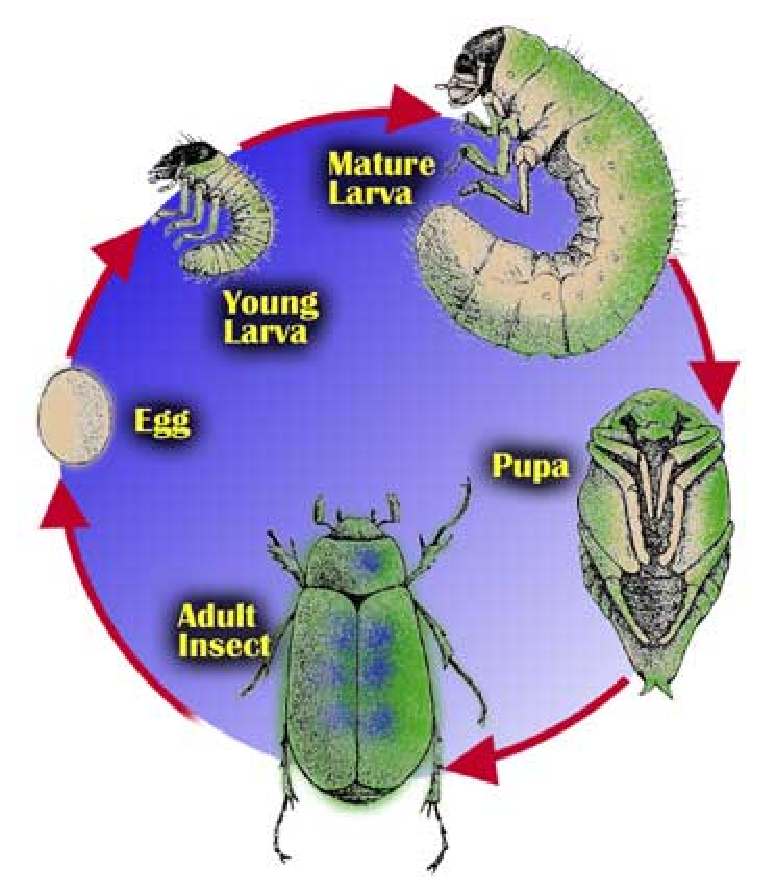
\includegraphics[width=.4\textwidth]{figs_steph/insect_life_cycle}
\caption{Example of insect life cycle.}
\end{center}
\end{figure}



\section{Insect populations}
Assume that adult females of a species produce offspring at a fixed period of time each year. A proportion of the offspring (juveniles) survives to adulhood, reproduces, and dies (nonoverlapping of generations). Let
\begin{itemize}
\item $j_t$ number of juveniles in years $t$
\item $a_t$ number of adult females in year $t$
\item $p$ number of juveniles that survive in year $t$
\item $f$ number of offspring produced per female
\item $r$ ratio of females to adults.
\end{itemize}
Using the definition of state variables and parameters given above, the model can be expressed as follows
$$a_{t+1}=prj_t$$
$$j_{t+1}=f a_{t+1}$$
The system can be condensed in an unique equation:
$$j_{t+1}=f prj_t$$
If the initial population $j_0$ of juveniles is known, the solution is unique and is
$$j_t=(f pr)^tj_0 \quad t=0,1,2,\dots$$
The asymptotic behavior of the solution depends on the value of $f pr$:
\begin{itemize}
\item If $f pr<1$ $\lim_{t\rightarrow +\infty} j_t=0$ extinction of the population,
\item If $f pr>1$ $\lim_{t\rightarrow +\infty} j_t=+\infty$ explosion of the population.
\end{itemize}


\section{Pharmacology}
A drug is administred once every four hours. Let $D_n$ be the amount of the drug in the blood system at the beginning of the $n^{th}$ interval.  The body eliminates a certain fraction $p$ of the drug during each time interval. If the amount administred is $D_0$, find $D_n$ and $\lim_{n\rightarrow\infty}D_{n}$.

The evolution of the concentration can be described by 
\[
D_{n+1}=D_n-pD_n +D_0=(1-p)D_n +D_0 \quad n=0,1,\dots,
\]
and the initial condition is $D_0$.
The equilibrium solution is $D^*=\frac{D_0}{p}$ (obtained by solving $D_{n}=(1-p)D_n +D_0$).
Using Proposition \ref{Prop:FirstLinNonH} the solution is unique and is
\[
D_n=(1-p)^n\left [D_0-\frac{D_0}{p}\right ] +\frac{D_0}{p} \quad n=0,1,2,\ldots
\]
The limiting behavior is
\[
\lim _{n\rightarrow +\infty}D_n=\frac{D_0}{p},
\]
since $(1-p)<1$.
Note that if a differential equation formalism were used, the system would take the form
$$\frac{dD}{dt}=-pD +D_0, \quad D(0)=D_0,$$
and the solution would be $D(t)=\frac{D_0}{p}+(D_0-\frac{D_0}{p})e^{-pt}$.

\section{Propagation of annual plants}
Plants produce seeds at the end of their growth season (August), after which they die. A fraction of these seeds survive the winter, and some of these germinate at the beginning of the season (May), giving rise to the new generation of plants. The fraction that germinates depends on the age of the seeds. 
\begin{itemize}
\item $\gamma$ number of seeds produced per plant in August
\item $\sigma$ fraction of seeds that survive a given winter
\item $\alpha$ fraction of one-year-old seeds that germinate in May
\item $\beta$ fraction of two-year-old seeds that germinate in May
\item Seeds older than two years are no longer viable
\end{itemize}

State variables:
\begin{itemize}
\item $p_n$ number of plants in generation $n$
\item $s_n$ number of new seed in generation $n$
\item $s^1_n$ number of one-year-old seeds in generation $n$
\item $s_{n}^{2}$ number of two-year-old seeds in generation $n$
\end{itemize}
Equations:
\begin{subequations}\label{eq:plant}
\begin{align}
p_n=&\alpha s^1_n+\beta s_{n}^{2}\label{eq:plant1}\\
s_{n}=&\gamma p_{n}\label{eq:plant2}\\
s_n^1=&\sigma s_{n-1}\label{eq:plant3}\\
s_{n}^{2}=&\sigma (1-\alpha)s^1_{n-1}\label{eq:plant4}
\end{align}   
\end{subequations} 
Condensing equations \eqref{eq:plant2}, \eqref{eq:plant3} and \eqref{eq:plant4} we obtain
$$s_n^1=\sigma \gamma p_{n-1}$$
and 
$$s_{n}^{2}=\sigma (1-\alpha)\sigma \gamma p_{n-2}$$
therefore, we can express the model as a system of 3 First-order difference equations
\begin{equation*}
\begin{array}{ll}
p_n=&\alpha s_n+\beta \sigma (1-\alpha)s_{n-1}\\
s_n^1=&\sigma \gamma p_{n-1}\\
s_{n}^{2}=&\sigma (1-\alpha)\sigma \gamma p_{n-2}
\end{array}
\end{equation*}
or as 1 Second-order equation:
\begin{equation}\label{eq:PLANTS}
p_n=\alpha \sigma \gamma p_{n-1}+\beta \sigma (1-\alpha)\sigma \gamma p_{n-2}
\end{equation}

The characteristic equation corresponding to the model \eqref{eq:PLANTS} is
$$\lambda ^2 - \alpha \sigma \gamma \lambda - \beta \sigma^2 (1-\alpha) \gamma=0.$$
Eigenvalues are
$$\lambda _{1,2}=\frac{\alpha \sigma \gamma \pm \sqrt{(\alpha \sigma \gamma)^2+4\beta \sigma^2 (1-\alpha) \gamma}}{2}$$
and
%=\frac{\alpha \sigma \gamma \pm \sigma\sqrt{(\alpha  \gamma)^2+4\beta  (1-\alpha) \gamma}}{2}
$$\lambda _{1,2}=\frac{\alpha \sigma \gamma }{2}\left (1\pm \sqrt{1+\frac{4\beta  (1-\alpha)}{\alpha^2 \gamma }}\right ).$$
%where $\delta = \frac{4\beta  (1-\alpha)}{\alpha^2 \gamma }$
The dominant eigenvalue (the eigenvalue corresponding to the solution that determines the limiting behavior of the general solution) is the positive eigenvalue
$$\lambda _{1}=\frac{\alpha \sigma \gamma }{2}\left (1+ \sqrt{1+\frac{4\beta  (1-\alpha)}{\alpha^2 \gamma }}\right ).$$
If $0<\lambda _1 <1$ the plant population will become extinct.
If $\lambda _1 >1$ the plant population will grow.






\section{Red blood cells}
In the circulatory system, red blood cells are constantly being destroyed and replaced. They carry oxygen throughout the body and they must be maintained at a constant level. The spleen filters out and destroys a fraction of the cells daily and the bone marrow produces a number proportional to the number lost on the previous day. The cell count on dat $t$ is modeled as followed:
\begin{itemize}
\item $R_t$ number of red blood cells in circulation on day $t$.
\item $M_t$ number of red blood cells produced by marrow on day $t$.
\item $f$ fraction of red blood cells removed by spleen, $0<f<1$.
\item $\gamma$ production constant, $\gamma >0$
\end{itemize}
The system of difference equations is
\begin{subequations}\label{eq:reblood}
\begin{align}
R_{t+1}=&(1-f)R_t+M_t\label{eq:reblood1}\\
M_{t+1}=&\gamma f R_t \label{eq:reblood2}
\end{align}   
\end{subequations} 
or a Second-order difference equation:
\begin{equation}\label{eq:BLOOD}
R_{t+1}=(1-f)R_t+\gamma f R_{t-1}
\end{equation}
Characteristic equation corresponding to the model \eqref{eq:BLOOD} is
$$\lambda ^2 - (1-f) \lambda -  \gamma f=0$$
Eigenvalues are
$$\lambda_{1,2}=\frac{(1-f)\pm \sqrt{(1-f)^2 + 4 \gamma f}}{2}$$

For homeostasis in the red blood cell count, the total number of red blood cell has to stay constant. Then the dominanting eigenvalue has to be $\lambda_1 =1$.

The dominating eigenvalue is 
$$\lambda_{1}=\frac{(1-f)+ \sqrt{(1-f)^2 + 4 \gamma f}}{2}.$$
By investigating $\lambda _1= 1$, we found that the condition, $\gamma =1$, has to be satisfied.


If $\gamma =1$, $\lambda _2= -f$, and the solution is
$$R_t= c_1 (-f^{t}) +c_2$$
the system is oscillating but decreasing in magnitude to reach a constant number.



\section{Killer whales}
Killer whales are long-lived marine mammals that live in stable
social groups called ``pods''. Demographic
data on killer whale populations in the coastal waters of British Columbia and Washington
state have been collected since 1973. Brault and Caswell (1993) used the 1973-1987 data and
a stage-structured matrix model to investigated several demographic questions concerning the
whales. They model the females with a mixed age-stage classification: yearlings, juveniles (past
the first year, but not mature), mature females, and post-reproductive females. 
$$
A =\left (\begin{array}{cccc}
0 & 0.0043 & 0.1132 & 0\\
0.9775 & 0.9111 & 0 & 0\\
0 & 0.0736 & 0.9534 & 0\\
0 & 0 & 0.0452 & 0.9804
\end{array}\right )$$
\begin{itemize}
\item Draw the life-cycle graph associated with the matrix A.
\item Computes the dominant eigenvalue. 
\item Find the stable stage distribution for the whale population.
\item Projects the population dynamics for the next 50 years assuming that the current population
vector is $x_0 = (10, 60, 110, 70)$ .
%(c) Plots on 3 separate graphs the projected changes over time in
%(i) N(t) = total population size in year t,
%(ii) the annual population growth rate .(t) = N(t + 1)/N(t),
%(iii) the proportion of individuals in each stage.
%Does the population structure become stable? How does it change over time? How quickly
%does the annual growth rate .(t) converge to the dominant eigenvalue .?
\end{itemize}

MatLab code:
\begin{verbatim}
L=[0 0.0043 0.1123 0;.9775 0.9111 0 0;0 .0736 0.9534 0;0 0 0.0452 0.9804];
x0=[10;60;110;70];
X=zeros(4,51);
X(:,1)=x0;
%simulations
for k=2:51, X(:,k)=L*X(:,k-1); end
t=0:50;
plot(t,X);
xlabel('Time');
ylabel('Population');
legend('Yearlings', 'Juveniles', 'Mature females','Post-reproductive females')
% limiting behavior
L=[0 0.0043 0.1123 0;.9775 0.9111 0 0;0 .0736 0.9534 0;0 0 0.0452 0.9804];
Value=eig(L);
dominant=max(Value)
[V,D]=eig(L)
\end{verbatim}

\begin{verbatim}
dominant =
    1.0251

V =
         0    0.0658   -0.0655    0.6788
         0    0.5640    0.8371   -0.7321
         0    0.5789   -0.5187    0.0568
    1.0000    0.5852    0.1609   -0.0026

D =
    0.9804         0         0         0
         0    1.0251         0         0
         0         0    0.8346         0
         0         0         0    0.0048

>> v1=V(:,2)/sum(V(:,2))

v1 =
    0.0367
    0.3144
    0.3227
    0.3262
\end{verbatim}

The dominant eigenvalue is $1.0251$, and the associated eigenvector is $(0.0658,0.5640,0.5789,0.5852)^T$. By summing all the entries of this eigenvector and by dividing each of its entries by this sum, we can express the stable stage distribution $v_1$ for the whale population.

\begin{center}
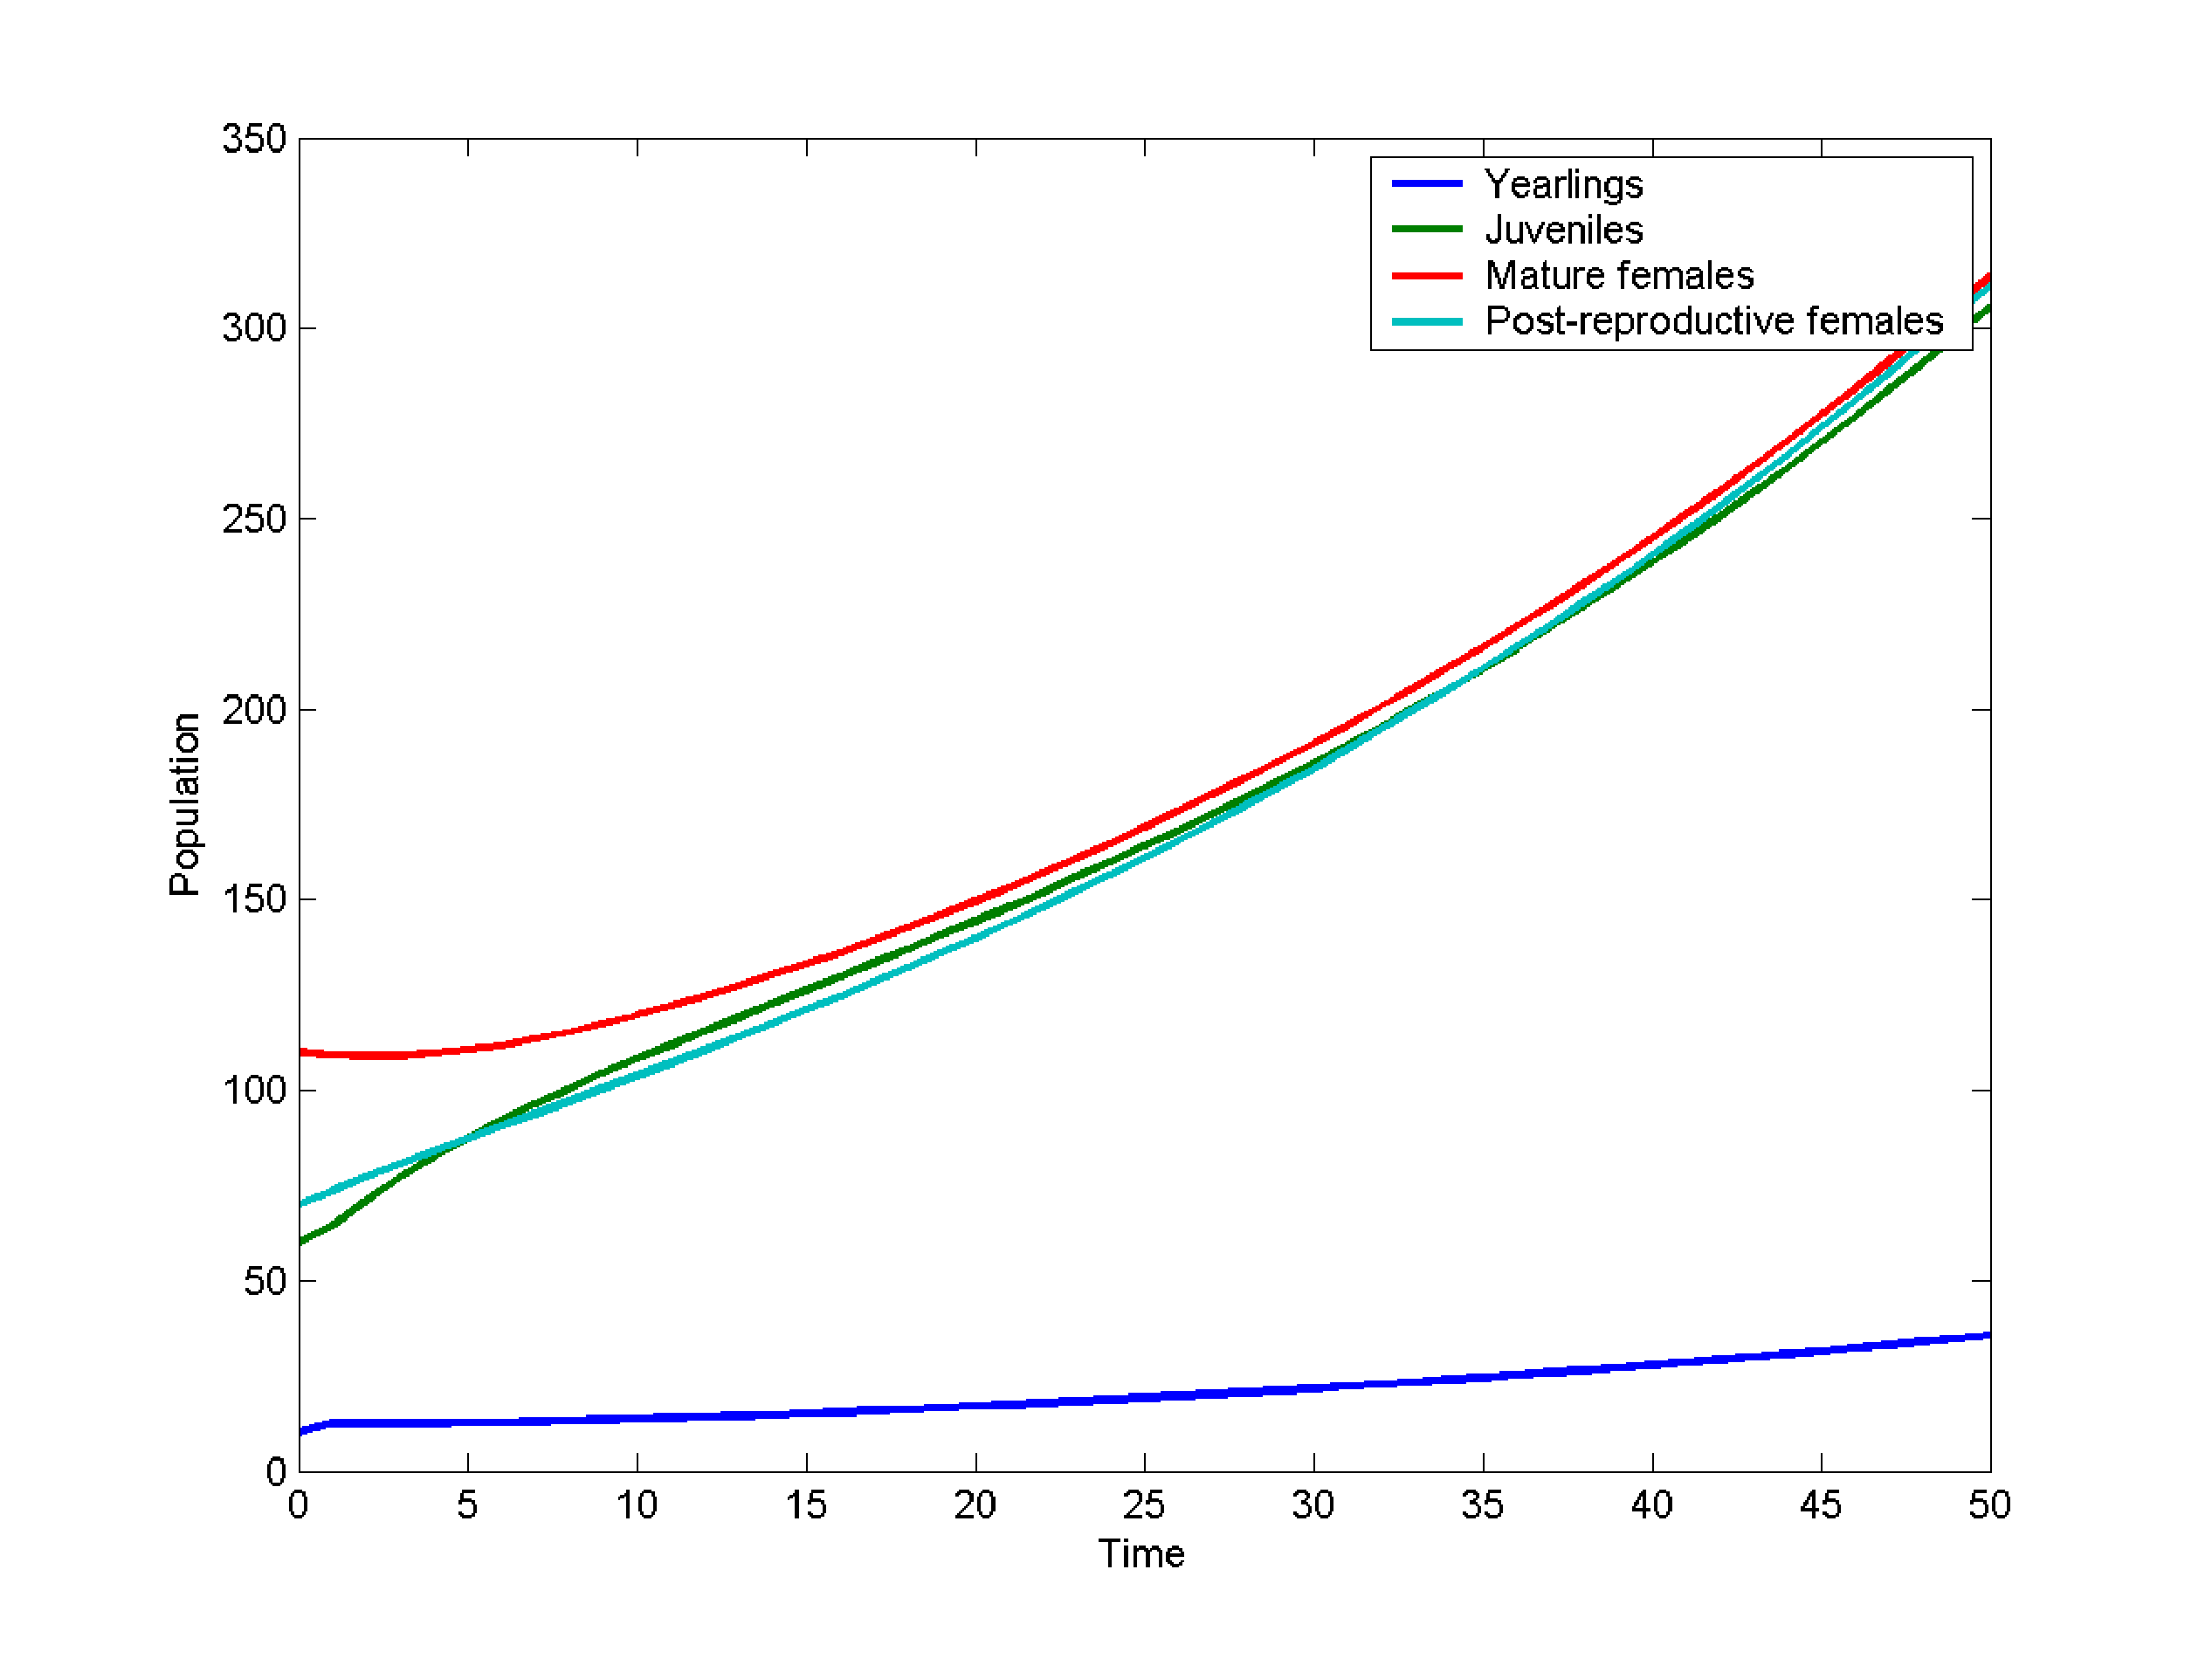
\includegraphics[width=.6\textwidth]{figs_steph/KillerWhales}
\end{center}














